%%
%% $Id$
%%
%% Copyright (c) 2007-2008 Christian Fehler
%% Copyright (c) 2007-2008 Benjamin Mies
%%


\chapter{Grammatiken}\label{Grammars}

Grammatiken gehören auch zu dem Punkten, welche in unser Lernwerkzeug mit
eingehen sollen. Der Benutzer muss die Möglichkeit haben eine Menge von
Terminalzeichen und Nichtterminalzeichen anzugeben, ebenso wie ein Startsymbol
festzulegen. Dies haben wir durch Eingabefeldern realisiert, hinter welchen
entsprechende Parser liegen. Die Parser werden detailiert im Kapitel
\ref{Parser} erläutert.

  \begin{figure}[h!]
  \begin{center}
  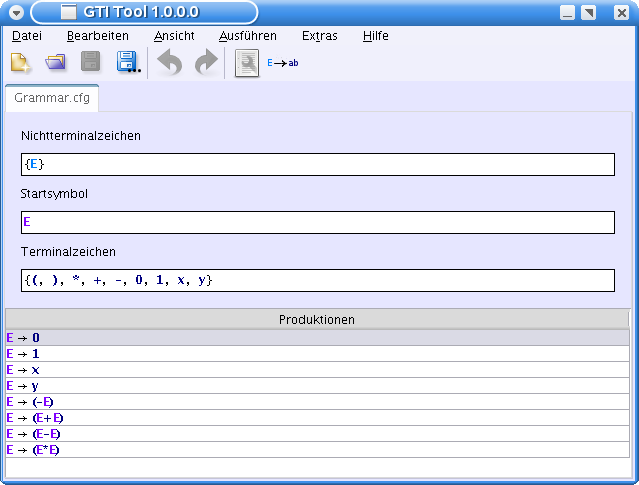
\includegraphics[width=12cm]{../images/cfg_example.png}
  \caption{Grammatik}
  \end{center}
  \end{figure}


Also fehlte noch die Darstellung der Produktionen. Hierbei haben wir uns für
eine Listenansicht entschieden, wobei die Produktionen als PrettyString
angezeigt werden. Das bedeutet, dass die verschiedenen Symbole
(Terminalzeichen, Nichtterminalzeichen, Startsymbol) in den Farben dargestellt
bekommt, die man in den Einstellungen dafür vergeben hat. Wir hoffen dadurch
eine bessere Übersichtlichkeit in den einzelnen Produktionen für den Benutzer
geschaffen zu haben.\vspace{10pt}

Als Hilfestellung beim Anlegen von neuen Produktionen wird die aktuelle
Konfiguration der Grammatik überhalb der existierenden Produktionen angezeigt.

  \begin{figure}[h!]
  \begin{center}
  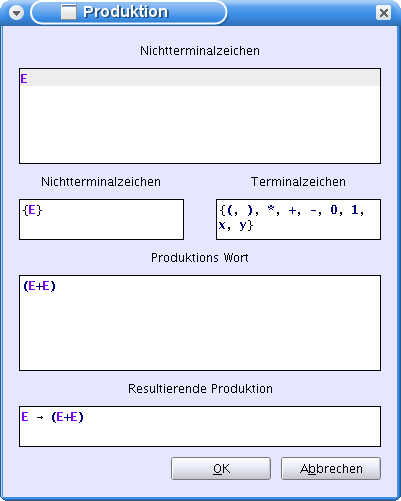
\includegraphics[width=8cm]{../images/production_dialog.png}
  \caption{Grammatik - Produktion anlegen}
  \end{center}
  \end{figure}


Wir haben versucht, das anlegen einer neuen Produktion so intuitiv wie möglich
zu gestalten. Der Benutzer kann das Nonterminal, welches die linke
Seite der Produktion repräsentiert, anhand einer Liste der
verfügbaren Symbole auswählen. Die Eingabe der Rechten Seite ist
wieder über ein Textfeld, mit entsprechendem Parser realisiert
worden. Oberhalb des Eingabefeldes wird dabei angezeigt, welche Symbole zur
Konstruktion des des Wortes der Satzform zur Verfügung stehen. Als weiter
Hilfestellung haben wir unterhalb des Eingabefeldes einen Bereich angelegt,
in welchem die resultierende Produktion angezeigt wird. So kann der
Benuzter zu jederzeit überprüfen, ob das Ergebnis seinen
Vorstellungen entspricht.\vspace{10pt}

Der Benutzer hat auch die Möglichkeit seine definierte Grammatik validieren zu
lassen. Wie das Validieren umgesetzt wurde und welche Möglichkeiten der
Benutzer dadurch hat wird in Kapitel \ref{Interaction} erläutert.
